\renewcommand{\theequation}{\theenumi}
\begin{enumerate}[label=\arabic*.,ref=\thesubsection.\theenumi]
\item Find the locus of a point which is equidistant from the points $\myvec{6\\-3}$, $\myvec{-4\\7}$.
\item Find the point on the line
\begin{align}
\myvec{2 & 5}\vec{x}+7=0
\end{align}
which is equidistant from the points $\myvec{2\\-3}$, $\myvec{-4\\1}$.
\item Find the coordinates of the circumcentre of the triangle whose corners are at the points $\myvec{4\\3}$, $\myvec{-1\\2}$, $\myvec{2\\-2}$.
\item Find the equations of the lines through $\myvec{3\\1}$ which are respectively parallel and perpendicular to the line joining the points $\myvec{2\\4}$, $\myvec{5\\-6}$.
\item Find the locus of a point at which the join of the points $\myvec{2\\1}$ and $\myvec{-3\\4}$ subtends a right angle.
\item Find the orthocentre of a triangle whose corners are at the points $\myvec{1\\2}$, $\myvec{-3\\-4}$, $\myvec{6\\2}$.
\item Prove that the line joining the points $\myvec{2\\-1}$, $\myvec{-3\\5}$ makes with the axes a triangle of area $\frac{49}{60}$.
\item $ABCD$ is a parallelogram and the coordinates of $\vec{A}$, $\vec{B}$ and $\vec{C}$ are $\myvec{2\\4}$, $\myvec{1\\2}$ and $\myvec{4\\1}$ Find the coordinates of $\vec{D}$.
\item Find the area of the triangle formed by the lines 
\numberwithin{equation}{enumi}
\begin{align}
\myvec{3&-2}\vec{x}=5
\\ 
\myvec{3 &4}\vec{x}=7
\\
\myvec{0 & 1}\vec{x}  +2 = 0
\end{align}
\item Find the centre of the inscribed circle of the triangle whose sides are
\begin{align}
\myvec{3&-4}\vec{x}&=0
\\
\myvec{ 12&-5}\vec{x}&=0,
\\ 
\myvec{4&3}\vec{x}&=8
\end{align}
\renewcommand{\theequation}{\theenumi}
\item The ends of a diagonal of a square are on the coordinate axes at the points $\myvec{2a\\0}$, $\myvec{0\\a}$.  Find the equations of the sides.
\item The sides of a triangle $ABC$ are
\begin{align}
AB=3, BC = 5, CA = 4
\end{align}
and $\vec{A}, \vec{B}$ are on the axes $OX$, $OY$ respectively, while $AC$ makes an angle $\theta$ with $OX$.  Prove that the locus of $\vec{C}$, as $\theta$ varies, is given by the equation
\begin{align}
\vec{x}^T\myvec{16 & -12\\-12 & 25}\vec{x} = 256
%16x^2-24xy+25y^2 = 256
\end{align}
\item Prove that the locus of a point at which the join of the points $\myvec{a\\0}$ and $\myvec{-a\\0}$ subtends an angle of $45\degree$ is
\begin{align}
\vec{x}^T\vec{x}-2a\myvec{0 & 1}\vec{x} = a^2
%x^2+y^2-2ay = a^2
\end{align}
\numberwithin{equation}{enumi}
\item Prove that the line
\begin{align}
\vec{n}^T\vec{x}+c=0
\end{align}
divides the line joining  the points $\vec{x}_1, \vec{x}_2$ in the ratio
\begin{align}
-\frac{\vec{n}^T\vec{x}_1+c}{\vec{n}^T\vec{x}_2+c}
\end{align}
\item Find the equation of the line joining the point $\vec{x}_1$, to the point of intersection of the lines
\begin{align}
\vec{n}^T\vec{x}+c=0
\\
\vec{n}_1^T\vec{x}+c_1=0
\end{align}
\item Find  the equations of the diagonals of the parallelogram whose sides are
\begin{align}
\vec{n}^T\vec{x}+c&=0
\\
\vec{n}^T\vec{x}+d&=0
\\
\vec{n}_1^T\vec{x}+c_1&=0
\\
\vec{n}_1^T\vec{x}+d_1&=0
\end{align}
%are
%{\small
%\begin{align}
%\brak{c_1-d_1}\brak{ax+by+c}-\brak{c-d}\brak{a_1x+b_1y+c_1} = 0
%\\
%\brak{c_1-d_1}\brak{ax+by+c}+\brak{c-d}\brak{a_1x+b_1y+c_1} = 0
%\\
%\brak{c-d}\brak{c_1-d_1}/\brak{ab_1-a_1b}.
%\end{align}
%}
\renewcommand{\theequation}{\theenumi}
\item Prove that for all values of $k$ the line
\begin{align}
\myvec{2+k &1-2k}\vec{x} + 5 = 0
\end{align}
passes through a fixed point, and find its coordinates.
\item Find the angle between the lines
\begin{align}
\vec{x}^T
\myvec{1 & -\sec \theta\\-\sec\theta & 1} 
\vec{x} = 0
\end{align}
\numberwithin{equation}{enumi}
\item Prove that the pairs of straight lines represented by
\begin{align}
\vec{x}^T
\myvec{1 & \frac{1}{2}\\\frac{1}{2} & 0} 
\vec{x} = 0
\\
\vec{x}^T
\myvec{6 & -\frac{1}{2}\\-\frac{1}{2} & -1} 
\vec{x} = 0
\end{align}
are such that the angles between one pair are equal to the angles between the other pair.
\renewcommand{\theequation}{\theenumi}
\item Find the angles between the lines
\begin{align}
x^3-3x^2y-3xy^2+y^3 = 0
\end{align}
\numberwithin{equation}{enumi}
\item Find the area of the triangle whose sides are given by
\begin{align}
\vec{x}^T
\myvec{1 & -{2}\\-{2} & 3} 
\vec{x} = 0
\\
\myvec{3&4}\vec{x}=7
\end{align}
\renewcommand{\theequation}{\theenumi}
\item Show that the equation 
\begin{align}
    \vec{x}^T\myvec{6&-\frac{1}{2}\\-\frac{1}{2}&-15}\vec{x}+\myvec{-11& 31}\vec{x}-10=0\label{eq:solutions/2/6/22/eq:1}
\end{align}
represents two straight lines,and find the equations of the bisectors of the angles between them.
%
%\item Show that the equation
%\begin{align}
%\vec{x}^T
%\myvec{6 & -\frac{1}{2}\\-\frac{1}{2} & -15} 
%\vec{x} 
%+\myvec{-11&31}\vec{x}-10=0
%\end{align}
%represents two straight lines, and find the equations of the bisectors of the angles between them.
\\
\solution

{construction}
Any quadratic equation in terms of $x,y$ of the form $ax^2+2bxy+cy^2+2dx+2ey+f=0$,can be written as
\begin{align}
    \vec{x}^T\vec{V}\vec{x}+2\vec{u}^T\vec{x}+f=0
%\label{eq:solutions/2/6/22/eq:2}
\\
    \text{where,}
    \vec{V}=\myvec{a&b\\b&c}\\
    \vec{u}=\myvec{d\\e}
\end{align}
The equation \eqref{eq:solutions/2/6/22/eq:1} represents two intersecting straight lines when
\begin{align}
    \mydet{\vec{V} & u\\u^T &f}=0\label{eq:solutions/2/6/22/eq:2}\\
    \mydet{\vec{V}}<0
\end{align}
{explanation}
From equation \eqref{eq:solutions/2/6/22/eq:1} we get
\begin{align}
    \vec{V}=\myvec{6&-\frac{1}{2}\\-\frac{1}{2}&-15}\\
    \vec{u}=\myvec{\frac{-11}{2}\\ \frac{31}{2}}\\
    f=-10
\end{align}
calculating the equation \eqref{eq:solutions/2/6/22/eq:2},we get
\begin{align}
    \myvec{6&-\frac{1}{2}&\frac{-11}{2}\\-\frac{1}{2}&-15&\frac{31}{2}\\\frac{-11}{2}&\frac{31}{2}&-10}\xleftrightarrow[]{R_3=R_3+R_2+R_1}\myvec{6&-\frac{1}{2}&\frac{-11}{2}\\-\frac{1}{2}&-15&\frac{31}{2}\\0&0&0}
\end{align}
Therefore the determinant $0$.And also the determinant of $\vec{V}$ is
\begin{align}
    \mydet{\vec{V}}&=\mydet{6&-\frac{1}{2}\\-\frac{1}{2}&-15}\\
    &=-90.25\\
    &<0
\end{align}
Therefore the given equation represents the equation of two straight lines which intersect.
{point of intersection}
The point of intersection of the straight lines is given by 
\begin{align}
    c&=-\vec{V}^{-1}\vec{u}
\end{align}
The inverse of $\vec{V}$ can be found by using rref of augmented matrix of the matrices $\vec{V}$ and $\vec{I}$
\begin{align}
    \myvec{6&-\frac{1}{2}&1&0\\-\frac{1}{2}&-15&0&1}\xleftrightarrow{R_2=12R_2+R_1}\myvec{6&-\frac{1}{2}&1&0\\0&-\frac{361}{2}&1&12}\\
    \myvec{6&-\frac{1}{2}&1&0\\0&1&-\frac{2}{361}&-\frac{24}{361}}\xleftrightarrow{R_1=R_1+\frac{R_2}{2}}\myvec{6&0&\frac{360}{361}&-\frac{12}{361}\\0&1&-\frac{2}{361}&-\frac{24}{361}}\\
    \vec{V}^{-1}=\myvec{\frac{60}{361}&-\frac{2}{361}\\-\frac{2}{361}&-\frac{24}{361}}\\
    c=-\myvec{\frac{60}{361}&-\frac{2}{361}\\-\frac{2}{361}&-\frac{24}{361}}\myvec{-\frac{11}{2}\\\frac{31}{2}}\\
    c=\myvec{1\\1}
\end{align}
Therefore the lines intersect at the point $\myvec{1\\1}$.
{eigenvectors}
The characteristic equation of the matrix $\vec{V}$ is
\begin{align}
    \mydet{\vec{V}-\lambda\vec{I}}&=0\\
    \mydet{6-\lambda&-\frac{1}{2}\\-\frac{1}{2}&-15-\lambda}&=0\\
    \lambda^2+9\lambda-90.25&=0
\end{align}
So the eigenvalues will be
\begin{align}
    \lambda_1=\frac{-1}{2}\brak{9+\sqrt{442}}\\
    \lambda_2=\frac{-1}{2}\brak{9-\sqrt{442}}
\end{align}
The eigen vectors will be in the nullspace of $\vec{V}-\lambda_1\vec{I}$ and $\vec{V}-\lambda_2\vec{I}$.The eigen vector corresponding to eigen value $\lambda_1$ will be
\begin{align}
    \vec{V}-\lambda_1\vec{I}=\myvec{6+\frac{1}{2}\brak{9+\sqrt{442}}&-\frac{1}{2}\\-\frac{1}{2}&-15+\frac{1}{2}\brak{9+\sqrt{442}}}\\
    =\myvec{\frac{1}{2}\brak{21+\sqrt{442}}&-\frac{1}{2}\\-\frac{1}{2}&\frac{1}{2}\brak{-21+\sqrt{442}}}\\
    \xleftrightarrow[]{R_2=\brak{21+\sqrt{442}}R_2+R_1}\myvec{\frac{1}{2}\brak{21+\sqrt{442}}&-\frac{1}{2}\\0&0}
\end{align}
The above reduced matrix has one free variable.Let it be $1$,then the eigen vector will be
\begin{align}
    {p_1}=\myvec{1\\21+\sqrt{442}}
\end{align}
normalizing $p_1$,we get
\begin{align}
    p_1=\frac{1}{\sqrt{884+42\sqrt{442}}}\myvec{1\\21+\sqrt{442}}
\end{align}
the eigen vector corresponding to eigen value $\lambda_2$ will be
\begin{align}
    \vec{V}-\lambda_1\vec{I}=\myvec{6+\frac{1}{2}\brak{9-\sqrt{442}}&-\frac{1}{2}\\-\frac{1}{2}&-15+\frac{1}{2}\brak{9-\sqrt{442}}}\\
    =\myvec{\frac{1}{2}\brak{21-\sqrt{442}}&-\frac{1}{2}\\-\frac{1}{2}&\frac{1}{2}\brak{-21-\sqrt{442}}}\\
    \xleftrightarrow[]{R_2=\brak{21-\sqrt{442}}R_2+R_1}\myvec{\frac{1}{2}\brak{21-\sqrt{442}}&-\frac{1}{2}\\0&0}
\end{align}
The above reduced matrix has one free variable.Let it be $1$,then the eigen vector will be
\begin{align}
    {p_2}=\myvec{1\\21-\sqrt{442}}
\end{align}
normalizing $p_2$,we get
\begin{align}
    p_2=\frac{1}{\sqrt{884-42\sqrt{442}}}\myvec{1\\21-\sqrt{442}}
\end{align}
So the transformation matrix will be 
\begin{align}
    \vec{P}=\myvec{p_1&p_2}=\myvec{\frac{1}{\sqrt{884+42\sqrt{442}}}&\frac{1}{\sqrt{884-42\sqrt{442}}}\\\frac{21+\sqrt{442}}{\sqrt{884+42\sqrt{442}}}&\frac{21-\sqrt{442}}{\sqrt{884-42\sqrt{442}}}}
\end{align}
{affine transformation}
Doing the affine transformation on given quadratic equation, we get pair to intersecting straight lines passing through origin.\par
Let the affine transformation be $\vec{x}=\vec{P}\vec{y}+c$.The transformation will be
\begin{align}
    \brak{\vec{P}\vec{y}+c}^T\vec{V}\brak{\vec{P}\vec{y}+c}+2\vec{u}^T\brak{\vec{P}\vec{y}+c}+f=0\\
\end{align}
    \begin{multline}
        \vec{y}^T\brak{\vec{P}^T\vec{V}\vec{P}}\vec{y}+2\brak{c^T\vec{V}+\vec{u}^T}\vec{P}\vec{y}\\
        +c^T\vec{V}c+2\vec{u}^Tc+f=0
\label{eq:solutions/2/6/22/eq:5}
    \end{multline}
\begin{figure}[t]
    \centering
    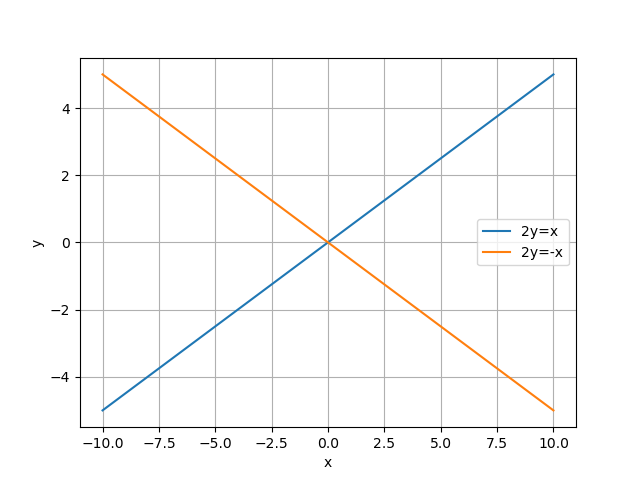
\includegraphics[width=\columnwidth]{./solutions/2/6/22/Fig1_a5.png}
    \caption{straight lines after affine transformation passing through origin}
    \label{eq:solutions/2/6/22/fig:1}
\end{figure}
if the point c is taken as the point of intersection of the two lines.
\begin{align}
    c^T\vec{V}c+2\vec{u}^Tc+f=0\\
    c^T\vec{V}+\vec{u}^T=0
\end{align}
So the affine transformation of the given lines will be
\begin{align}
    \vec{y}^T\brak{\vec{P}^T\vec{V}\vec{P}}\vec{y}=0\\
    \vec{y}^T\myvec{-1.5&0\\0&6}\vec{y}=0\\
    \brak{x-2y}\brak{x+2y}=0
\end{align}
Since the two lines are symmetric with respect to both $X-axis$ and $Y-axis$,the axes themselves are the bisectors of the transformed pair of lines.So the bisectors will be $x=0$ and $y=0$.
Matrix notation will be of the form
\begin{align}
    \vec{y}^T\myvec{0&0.5\\0.5&0}\vec{y}=0\\
    \vec{y}^T\vec{K}\vec{y}=0\\
    \vec{K}=\myvec{0&0.5\\0.5&0}
\end{align}
{bisectors}
Taking the inverse of the affine transformation of the equation $xy=0$,will give the angle bisectors.
\begin{align}
    \brak{\vec{P}^{-1}\vec{x}-\vec{P}^{-1}c}^T\vec{K}\brak{\vec{P}^{-1}\vec{x}-\vec{P}^{-1}c}=0\\
    \vec{x}^T\vec{P}\vec{K}\vec{P}^T\vec{x}-2c^T\vec{P}\vec{K}\vec{P}^T\vec{x}+c^T\vec{P}\vec{K}\vec{P}^Tc=0
\end{align}
Substituting the values we get
    \begin{multline}
        \vec{x}^T\myvec{\frac{1}{2\sqrt{442}}&\frac{21}{2\sqrt{442}}\\\frac{21}{2\sqrt{442}}&-\frac{1}{2\sqrt{442}}}\vec{x}\\
        -\myvec{\frac{22}{\sqrt{442}}&\frac{20}{\sqrt{442}}}\vec{x}+\frac{21}{\sqrt{442}}=0
    \end{multline}
    \begin{multline}
        \frac{x^2}{2\sqrt{442}}+\frac{21}{\sqrt{442}}xy-\frac{y^2}{2\sqrt{442}}\\
        -\frac{22x}{\sqrt{442}}-\frac{20y}{\sqrt{442}}+\frac{21}{\sqrt{442}}=0
    \end{multline}\\
\begin{align}
    x^2+42xy-y^2-44x-40y+42=0
\end{align}
Therefore the equation of bisectors of the given line in quadratic form is
\begin{align}
    \vec{x}^T\myvec{1&21\\21&-1}\vec{x}-\myvec{44&40}\vec{x}+42=0
\end{align}
\begin{figure}[t]
    \centering
    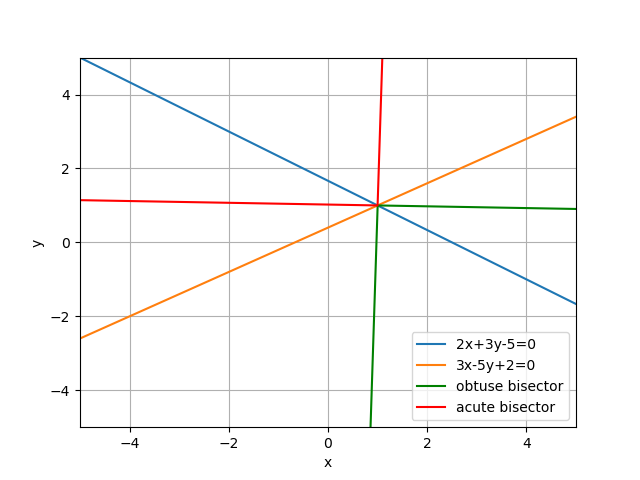
\includegraphics[width=\columnwidth]{./solutions/2/6/22/Fig2_a5.png}
    \caption{Par of straight lines and their angular bisectors}
    \label{eq:solutions/2/6/22/fig:my_label}
\end{figure}

\item For what value of $k$ does the equation
\begin{align}
\vec{x}^T
\myvec{12 & \frac{7}{2}\\\frac{7}{2} & k} 
\vec{x} 
+\myvec{13&-1}\vec{x}+3=0
\end{align}
represent two straight lines? What is the angle between them?

\item For what value of $k$ does the equation 
\begin{equation} \label{eq:solutions/2/6/24/eq:1.1}
\vec{x}^T \myvec{6 && k/2 \\ k/2 && -3} \vec{x} + \myvec{4 && 5}\vec{x} -2 = 0
\end{equation}
represent a pair of straight lines?
\\
%\item For what values of $k$ does the equation
%\begin{align}
%\vec{x}^T
%\myvec{6 & \frac{k}{2}\\\frac{k}{2} & -3} 
%\vec{x} 
%+\myvec{4&5}\vec{x}-2=0
%\end{align}
%represent two straight lines?
\solution
\eqref{eq:solutions/2/6/24/eq:1.1} can also be written as 
\begin{equation}\label{eq:solutions/2/6/24/eq:2.1}
\vec{x}^T \myvec{a && b \\ b && c} \vec{x} + \myvec{d && e}\vec{x} + f = 0
\end{equation}
\begin{equation}\label{eq:solutions/2/6/24/eq:2.2}
\begin{split}
\vec{V}=\myvec{6 && k/2\\ k/2 && -3}\\
\vec{u}=\myvec{2\\5/2}\\
f= -2
\end{split}
\end{equation}
Block Matrix
\begin{equation} \label{eq:solutions/2/6/24/eq:2.3}
 = \myvec{6 && k/2 && 2\\ k/2 && -3 && 5/2\\2 && 5/2 && -2}
\end{equation} 
Determinant of the Block Matrix
\begin{equation} \label{eq:solutions/2/6/24/eq:2.4}
\Delta = \mydet{6 && k/2 && 2\\ k/2 && -3 && 5/2\\2 && 5/2 && -2}
\end{equation}
If the \eqref{eq:solutions/2/6/24/eq:1.1} represents a pair of straight lines\\
then the Determinant is zero
\begin{equation} \label{eq:solutions/2/6/24/eq:2.5}
\begin{split}
\Delta = 0\\
\implies \mydet{6 && k/2 && 2\\ k/2 && -3 && 5/2\\2 && 5/2 && -2} = 0\\
\implies 6\times(6-25/4)-k/2(-k-5)+2(5k/4+6) = 0\\
\implies k^2 + 10k + 21 = 0
\end{split}
\end{equation}
\begin{equation} \label{eq:solutions/2/6/24/eq:2.6}
\begin{split} 
\implies \boxed{ k = -3 }\\
\implies \boxed{ k = -7 }
\end{split}
\end{equation}
Substituting k=-3 in \eqref{eq:solutions/2/6/24/eq:1.1}
\begin{equation} \label{eq:solutions/2/6/24/eq:2.7}
\vec{x}^T \myvec{6 && -3/2 \\ -3/2 && -3} \vec{x} + \myvec{4 && 5}\vec{x} -2 = 0
\end{equation}
\eqref{eq:solutions/2/6/24/eq:2.2} can be represented as 
\begin{equation} \label{eq:solutions/2/6/24/eq:2.8}
\begin{split}
\vec{V}=\myvec{6 && -3/2\\ -3/2 && -3}\\
\vec{u}=\myvec{2\\5/2}\\
f= -2
\end{split}
\end{equation}
To find the separate equations of the straight lines we will use spectral decomposition.\\
Characteristic equation of $\vec{V}$ is given by:
\begin{equation} \label{eq:solutions/2/6/24/eq:2.9}
\begin{split}
\mydet{V-\lambda \vec{I}}=\mydet{6-\lambda && -3/2\\ -3/2 && -3-\lambda} = 0\\
\implies \lambda^2 - 3\lambda - 81/4 = 0
\end{split}
\end{equation}
The Eigen Values of $\vec{V}$ are:
\begin{equation} \label{eq:solutions/2/6/24/eq:2.10}
\lambda_1 = \frac{3+3\sqrt{10}}{2}, \lambda_2 = \frac{3-3\sqrt{10}}{2}
\end{equation}
Let $\vec{p}_1$ and $\vec{p}_2$ be the Eigen vector corresponding to $\lambda_1$ and $\lambda_2$ respectively\\
Eigen vector $\vec{p}$ is given as:
\begin{equation} \label{eq:solutions/2/6/24/eq:2.11}
\begin{split}
\vec{V}\vec{p} = \lambda\vec{p}\\
\implies (\vec{V} - \lambda \vec{I})\vec{p} = 0
\end{split}
\end{equation}
For $\lambda_1 = \frac{3+3\sqrt{10}}{2}$
\begin{equation}\label{eq:solutions/2/6/24/eq:2.12}
(\vec{V} - \lambda_1 \vec{I}) = \myvec{\frac{9-3\sqrt{10}}{2} && -3/2\\ -3/2 && \frac{-9-3\sqrt{10}}{2}}
\end{equation}
To find $ \vec{p}_1 $ Use Augmented Matrix of $(\vec{V} - \lambda \vec{I})$
\begin{equation} \label{eq:solutions/2/6/24/eq:2.13}
\begin{split}
 \myvec{\frac{9-3\sqrt{10}}{2} && -3/2 && 0\\ -3/2 && \frac{-9-3\sqrt{10}}{2} && 0}\\
\xleftrightarrow[]{R_1\rightarrow \frac{2}{9-3\sqrt{10}}R_1} 
\myvec{1 && 3+\sqrt{10} && 0\\ -3/2 && \frac{-9-3\sqrt{10}}{2} && 0}\\
\xleftrightarrow[]{R_1\rightarrow 3/2R_1+R_2} 
\myvec{1 && 3+\sqrt{10} && 0\\ 0 && 0 && 0} 
\end{split}
\end{equation}
So we get,
\begin{equation}\label{eq:solutions/2/6/24/eq:2.14}
x_1 + (3+\sqrt{10})x_2 = 0
\end{equation}
Therefore, Eigen Vector corresponding to $\lambda_1$
\begin{equation}\label{eq:solutions/2/6/24/eq:2.15}
\vec{p}_1 =\frac{1}{\sqrt{20+6\sqrt{10}}} \myvec{-(3+\sqrt{10}) \\ 1}
\end{equation}
Similarly for $\lambda_2 = \frac{3-3\sqrt{10}}{2}$
\begin{equation}\label{eq:solutions/2/6/24/eq:2.16}
\vec{p}_2 =\frac{1}{\sqrt{20-6\sqrt{10}}} \myvec{-(3-\sqrt{10}) \\ 1}
\end{equation}
We know that $\vec{V} = \vec{P}\vec{D}\vec{P}^T$ where $\vec{P}$ and $\vec{V}$ are given by:
\begin{equation} \label{eq:solutions/2/6/24/eq:2.17}
\begin{split}
\vec{D} = \myvec{\lambda_1 && 0\\ 0 && \lambda_2}\\
\implies \vec{D} = \myvec{\frac{3+3\sqrt{10}}{2} && 0\\ 0 &&\frac{3-3\sqrt{10}}{2} }
\end{split}
\end{equation}
Hence the rotation matrix P is
\begin{equation} \label{eq:solutions/2/6/24/eq:2.18}
\begin{split}
\vec{P} = \myvec{\vec{p}_1 && \vec{p}_2}\\
\implies \vec{P} = \myvec{\frac{-(3+\sqrt{10})}{\sqrt{20+6\sqrt{10}}} && \frac{-(3-\sqrt{10})}{\sqrt{20-6\sqrt{10}}} \\ \frac{1}{\sqrt{20+6\sqrt{10}}} && \frac{1}{\sqrt{20-6\sqrt{10}}}}
\end{split}
\end{equation}
We know that 
\begin{equation} \label{eq:solutions/2/6/24/eq:2.19}
\myvec{\sqrt{|\lambda_1|} && \sqrt{|\lambda_2|}}\vec{P}^T(\vec{x}-\vec{c}) = 0
\end{equation}
where $\vec{c}$ is the point of intersection of the lines 
\begin{equation} \label{eq:solutions/2/6/24/eq:2.20}
\begin{split}
\vec{V}\vec{c} = -\vec{u}\\
\myvec{6 && -3/2\\-3/2 && -3} \vec{c} = -\myvec{2 \\ 5/2}\\
\implies \vec{c} = \myvec{-1/9 \\ 8/9}
\end{split}
\end{equation}
Substituting values in \eqref{eq:solutions/2/6/24/eq:2.19}
\begin{equation} \label{eq:solutions/2/6/24/eq:2.21}
\begin{split}
\myvec{ \sqrt{\frac{3+3\sqrt{10}}{2}} && \pm\sqrt{\frac{3-3\sqrt{10}}{2}}} \times \\
\myvec{ -\frac{3+\sqrt{10}}{\sqrt{20+6\sqrt{10}}} && \frac{1}{\sqrt{20+6\sqrt{10}}} \\ -\frac{3-\sqrt{10}}{\sqrt{20-6\sqrt{10}}} && -\frac{1}{\sqrt{20-6\sqrt{10}}}} \times \\
\myvec{x+1/9 \\ y-8/9}  = 0
\end{split}
\end{equation}
Simplifying \eqref{eq:solutions/2/6/24/eq:2.21} we get 
\begin{equation}\label{eq:solutions/2/6/24/eq:2.22}
\begin{split}
3x - 3y + 3 = 0 ~and~ 2x + y - 2/3 = 0\\
\boxed{(3x - 3y + 3)(2x + y - 2/3) = 0}
\end{split}
\end{equation}
Similarly substituting k=-7 in \eqref{eq:solutions/2/6/24/eq:1.1}
\begin{equation}\label{eq:solutions/2/6/24/eq:2.23}
\vec{x}^T \myvec{6 && -7/2 \\ -7/2 && -3} \vec{x} + \myvec{4 && 5}\vec{x} -2 = 0
\end{equation}
Equation \eqref{eq:solutions/2/6/24/eq:2.2} can be represented as 
\begin{equation} \label{eq:solutions/2/6/24/2.24}
\begin{split}
\vec{V}=\myvec{6 && -7/2\\ -7/2 && -3}\\
\vec{u}=\myvec{2\\5/2}\\
f= -2
\end{split}
\end{equation}
To find the separate equations of the straight lines we will use spectral decomposition.\\
Characteristic equation of $\vec{V}$ is given by:
\begin{equation} \label{eq:solutions/2/6/24/2.25}
\begin{split}
\mydet{V-\lambda \vec{I}}=\mydet{6-\lambda && -7/2\\ -7/2 && -3-\lambda} = 0\\
\implies \lambda^2 - 3\lambda - 121/4 = 0
\end{split}
\end{equation}
The Eigen Values of $\vec{V}$ are:
\begin{equation} \label{eq:solutions/2/6/24/2.26}
\lambda_1 = \frac{3+\sqrt{130}}{2}, \lambda_2 = \frac{3-3\sqrt{130}}{2}
\end{equation}
Let $\vec{p}_1$ and $\vec{p}_2$ be the Eigen vector corresponding to $\lambda_1$ and $\lambda_2$ respectively\\
Eigen vector $\vec{p}$ is given as:
\begin{equation} \label{eq:solutions/2/6/24/2.27}
\begin{split}
\vec{V}\vec{p} = \lambda\vec{p}\\
\implies (\vec{V} - \lambda \vec{I})\vec{p} = 0
\end{split}
\end{equation}
For $\lambda_1 = \frac{3+\sqrt{130}}{2}$
\begin{equation}\label{eq:solutions/2/6/24/2.28}
(\vec{V} - \lambda_1 \vec{I}) = \myvec{\frac{9-\sqrt{130}}{2} && -7/2\\ -7/2 && \frac{-9-\sqrt{130}}{2}}
\end{equation}
To find $ \vec{p}_1 $ Use Augmented Matrix of $(\vec{V} - \lambda \vec{I})$
\begin{equation} \label{eq:solutions/2/6/24/2.29}
\begin{split}
 \myvec{\frac{9-\sqrt{130}}{2} && -7/2 && 0\\ -7/2 && \frac{-9-\sqrt{130}}{2} && 0}\\
\xleftrightarrow[]{R_1\rightarrow \frac{2}{9-\sqrt{130}}R_1} 
\myvec{1 && \frac{9+\sqrt{130}}{7} && 0\\ -7/2 && \frac{-9-\sqrt{130}}{2} && 0}\\
\xleftrightarrow[]{R_1\rightarrow 7/2R_1+R_2} 
\myvec{1 && \frac{9+\sqrt{130}}{7} && 0\\ 0 && 0 && 0} 
\end{split}
\end{equation}
So we get,
\begin{equation} \label{eq:solutions/2/6/24/2.30}
x_1 + (\frac{9+\sqrt{130}}{7})x_2 = 0
\end{equation}
Therefore, Eigen Vector corresponding to $\lambda_1$
\begin{equation} \label{eq:solutions/2/6/24/2.31}
\vec{p}_1 =\frac{7}{\sqrt{260+18\sqrt{130}}} \myvec{-\frac{9+\sqrt{130}}{7}) \\ 1}
\end{equation}
Similarly for $\lambda_2 = \frac{3-\sqrt{130}}{2}$
\begin{equation}\label{eq:solutions/2/6/24/2.32}
\vec{p}_2 =\frac{7}{\sqrt{260-18\sqrt{130}}} \myvec{-\frac{9-\sqrt{130}}{7} \\ 1}
\end{equation}
We know that $\vec{V} = \vec{P}\vec{D}\vec{P}^T$ where $\vec{P}$ and $\vec{V}$ are given by:
\begin{equation}\label{eq:solutions/2/6/24/2.33}
\vec{D} = \myvec{\lambda_1 && 0\\ 0 && \lambda_2}\\
\implies \vec{D} = \myvec{\frac{3+\sqrt{130}}{2} && 0\\ 0 &&\frac{3-\sqrt{130}}{2} }
\end{equation}
Hence the rotation matrix P is
\begin{equation} \label{eq:solutions/2/6/24/2.34}
\vec{P} = \myvec{\vec{p}_1 && \vec{p}_2}
\end{equation}
\begin{equation} \label{eq:solutions/2/6/24/2.35}
\implies \vec{P} = \myvec{-\frac{63+7\sqrt{130}}{\sqrt{260+18\sqrt{130}}} && -\frac{63-7\sqrt{130}}{\sqrt{260-18\sqrt{130}}} \\ \frac{7}{\sqrt{260+18\sqrt{10}}} && \frac{7}{\sqrt{260-18\sqrt{130}}}}
\end{equation}
We know that 
\begin{equation}\label{eq:solutions/2/6/24/2.36}
\myvec{\sqrt{|\lambda_1|} && \sqrt{|\lambda_2|}}\vec{P}^T(\vec{x}-\vec{c}) = 0
\end{equation}
where $\vec{c}$ is the point of intersection of the lines 
\begin{equation} \label{eq:solutions/2/6/24/2.37}
\begin{split}
\vec{V}\vec{c} = -\vec{u}\\
\myvec{6 && -7/2\\-7/2 && -3} \vec{c} = -\myvec{2 \\ 5/2}\\
\implies \vec{c} = \myvec{1/11 \\ 8/11}
\end{split}
\end{equation}
Substituting values in \eqref{eq:solutions/2/6/24/2.36}
\begin{equation} \label{eq:solutions/2/6/24/2.38}
\begin{split}
\myvec{ \sqrt{\frac{3+\sqrt{130}}{2}} && \pm\sqrt{\frac{3-\sqrt{130}}{2}}} \times \\
\myvec{ -\frac{63+7\sqrt{130}}{\sqrt{260+18\sqrt{130}}} && \frac{7}{\sqrt{260+18\sqrt{130}}} \\ -\frac{63-7\sqrt{130}}{\sqrt{260-18\sqrt{130}}} && \frac{7}{\sqrt{260-18\sqrt{130}}}} \times \\
\myvec{x-1/11 \\ y-8/11} = 0
\end{split}
\end{equation}
Simplifying \eqref{eq:solutions/2/6/24/2.38} we get 
\begin{equation} \label{eq:solutions/2/6/24/2.39}
\begin{split}
2x - 3y + 2 = 0~ and ~3x + y - 1 = 0\\
\boxed{(2x - 3y + 2)(3x + y - 1) = 0}
\end{split}
\end{equation}
\begin{figure}[!htb]
   \centering
   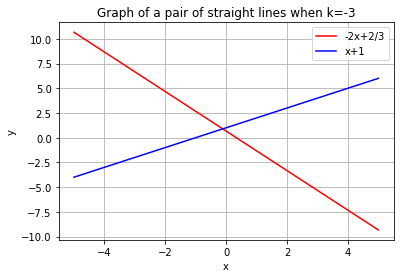
\includegraphics[width=\columnwidth]{solutions/2/6/24/fig1.png}
   \caption{Pair of straight lines when k=-3}
   \label{eq:solutions/2/6/24/fig:1}
\end{figure}
\begin{figure}[!htb]
   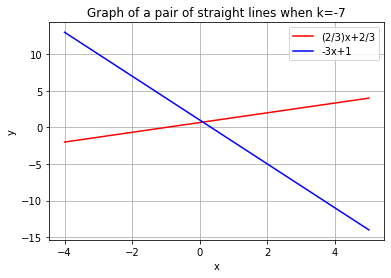
\includegraphics[width=\columnwidth]{solutions/2/6/24/fig2.png}
   \caption{Pair of straight lines when k=-7}
   \label{eq:solutions/2/6/24/fig:2}
\end{figure}

%
\end{enumerate}
